\chapter{Metodologia}
\label{cap:Metodologia}

Neste capítulo serão apresentadas as duas estratégias propostas e desenvolvidas nesta dissertação para o problema de dobramento de proteínas. A primeira trata-se de uma abordagem multi-objetiva utilizando dois algoritmos evolucionários multi-objetivos (AEMOs) para o PDP. Já a segunda visa aplicação da evolução gramatical  para gerar heurísticas de alto nível para um \textit{framework} hiper-heurístico  para PDP intitulada EGHyPDP.


O problema PDP simplificado foi modelado utilizando a representação relativa, descrita na subseção \ref{subsubsection:modeloHP}, afim de codificar as possíveis conformações de proteínas em vetores de inteiros. Segundo o estudo realizado por Krasnogor et al. \cite{krasnogor1999protein} esta representação possui um maior potencial em conduzir os algoritmos a resultados melhores. Cada gene do cromossomo especifica a direção que o amino ácido atual deve ser posicionado. Cada amino ácido é posicionado na direção especificada pelo respectivo gene em relação ao amino ácido anterior. O genes podem assumir apenas 3 valores (0,1 e 2): 0 indica que o próximo amino ácido deve ser posicionado à direita do amino ácido anterior, 1 indica que o próximo amino ácido deve ser posicionado à frente do amino ácido anterior e 2 indica que o próximo aminoácido deve ser posicionado à esquerda. 

A Figura \ref{img:cromossomo} apresenta um exemplo de um cromossomo hipotético e a conformação gerada no \textit{grid} para o modelo HP-2D.


\begin{figure}[!htb]
	\centering
	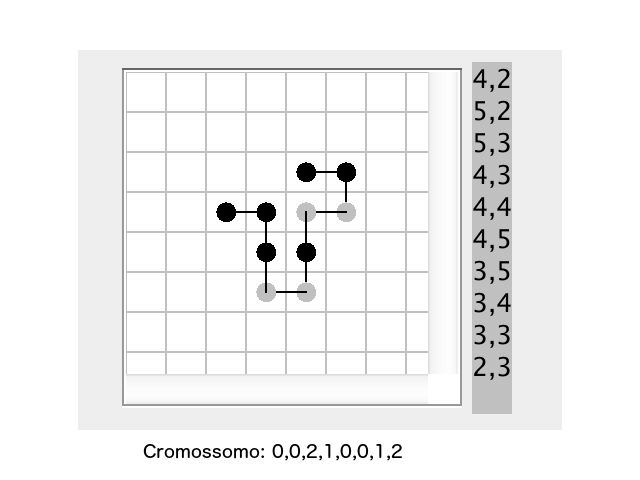
\includegraphics[scale=0.36]{Imagens/DecodedCromossome.png}
	\caption{Cromossomo decodificado que representa uma possível conformação para a cadeia HHPPHPPHHH}
	\label{img:cromossomo}
\end{figure}



Para ambas as abordagens o mesmo conjunto de heurísticas de baixo nível (operadores de cruzamento/mutaçào e busca locais) foi selecionado a partir dos estudos anteriores. O conjunto de heurísticas de baixo nível será descrito abaixo:

 \begin{itemize}
 	
 		\item \textit{Single Point Crossover} (1X): Este operador seleciona, de maneria aleatória, 1 ponto de cruzamento dividindo os indivíduos em 2 partes. Os genes entre as posições selecionadas são trocados entre os pais de modo a gerar dois novos filhos \cite{benitez2015algoritmo}.
 	
 	\item \textit{Two Points Crossover} (2X): Este operador seleciona, de maneria aleatória, 2 pontos de cruzamento dividindo os indivíduos em 3 partes. Os genes entre as posições selecionadas são trocados entre os pais de modo a gerar dois novos filhos \cite{benitez2015algoritmo}, conforme apresentado na figura \ref{fig:twopointscrossover}.
 	
 	
 	\begin{figure}[!htb]
 		\centering
 		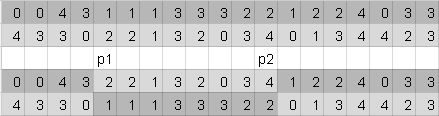
\includegraphics{Imagens/TwoPointsCrossover.png}
 		\caption{Exemplo de aplicação do operador 2x. \\Fonte Autoria Própria}
 		\label{fig:twopointscrossover}
 	\end{figure}
 	
 	
 	
 	
 	\item \textit{Multi Points Crossover} (MPX): Semelhante ao 2X porém com c pontos, baseado na função $c = int(n * 0.1)$, $n$ é o tamanho da sequência. O operador MPX é utilizado para promover diversidade estrutural realizando uma mescla randômica entre os pais, embora não tão radical quanto o \textit{Uniform  Crossover} \cite{sabar2014automatic}. Um exemplo de aplicação do operador MPX é apresentado na imagem \ref{fig:multipointscrossover}
 	
 	
 	\begin{figure}[!htb]
 		\centering
 		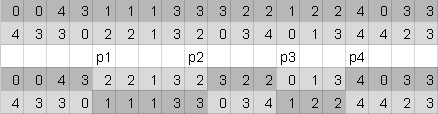
\includegraphics{Imagens/MultiPointsCrossover.png}
 		\caption{Exemplo de aplicação do operador MPX. \\Fonte Autoria Própria}
 		\label{fig:multipointscrossover}
 	\end{figure}
 	\item \textit{Segment Mutation} (SMUT): Altera um número aleatório (5 a 7) de genes consecutivos para direções distintas. Esta heurística introduz grandes mudanças na conformação, e tem uma grande probabilidade de criar colisões. Um mecanismo de reparação simples é aplicado no descendente gerado. A imagem \ref{fig:segmentMutation} apresenta um exemplo da aplicação do SMUT.
 	
 	\begin{figure}[!htb]
 		\centering
 		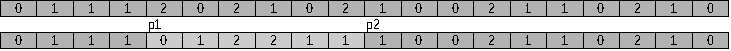
\includegraphics{Imagens/segmentMutation.png}
 		\caption{Exemplo de aplicação do operador SMUT. \\Fonte Autoria Própria}
 		\label{fig:segmentMutation}
 	\end{figure}
 	
 	
 	\item \textit {Exhaustive Search Mutation} (EMUT): Esta heurística seleciona um gene aleatório e testa todas as outras direções possíveis e irá manter a alteração que conseguir aumentar a qualidade da conformação. O \textit{tradeoff} deste operador é demandar 4 avaliações de \textit{fitness}, as quais devem ser levadas em consideração. Esta heurística tem grande potencial de melhorar o \textit{fitness} de uma conformação. 
 	
 	
 	\item \textit{Local Move Operator} (LM): Esta heurística troca direções entre dois genes aleatórios consecutivos. Existem algumas condições para que esta heurística possa ser executada, por exemplo, as novas direções não podem criar movimentos redundantes. Este operador introduz um "movimento de esquina". A figura \ref{fig:localMoveOperator} apresenta um exemplo da aplicação do operador LM. 
 	
 	
 	\begin{figure}[!htb]
 		\centering
 		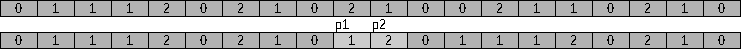
\includegraphics{Imagens/LocalMoveOperator.png}
 		\caption{Exemplo de aplicação do operador LM. \\Fonte Autoria Própria}
 		\label{fig:localMoveOperator}
 	\end{figure}
 	
 	
 	\item \textit{Loop Move Operator} (LPM): Da mesma maneira que a heurística LM, esta heurística troca direções entre dois genes que estão a 5 genes de distância na sequência, criando um movimento de \textit{loop}. A figura  \ref{fig:loopMoveOperator} apresenta um exemplo da aplicação do operador LPM.
 	
 	
 	\begin{figure}[!htb]
 		\centering
 		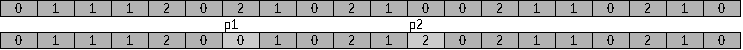
\includegraphics{Imagens/LoopMoveOperator.png}
 		\caption{Exemplo de aplicação do operador LPM. \\Fonte Autoria Própria}
 		\label{fig:loopMoveOperator}
 	\end{figure}
 	
 	\item \textit{Opposite Mutation} (OM): Esta heurística troca as direções, para direção oposta, de uma sequência de genes entre dois genes $(i,j)$ selecionados de maneira aleatória. A direção 0 ($F$) não possui oposta, portanto é mantida. Para exemplificar, suponha esta solução hipotética para uma sequência de 5 aminoácidos: $\{0,1,2,1,2\}$. Ela se tornaria $\{0,2,1,2,1\}$. A figura \ref{fig:oppositeMutation} apresenta um exemplo da aplicação do operador OM.
 	
 	
 	\begin{figure}[!htb]
 		\centering
 		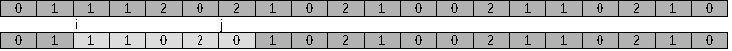
\includegraphics{Imagens/OppositeMutation.png}
 		\caption{Exemplo de aplicação do operador OM. \\Fonte Autoria Própria}
 		\label{fig:oppositeMutation}
 	\end{figure}
 	
 	
 	
 \end{itemize} 



 Este capítulo está divido em duas seções respectivamente para cada melhor apresentar as estratégias propostas nesta dissertação (AEMOs e o EGHyPDP). A seção \ref{sec:aemos} apresenta a estratégia multi objetiva onde foi utilizada dois algoritmos evolucionários, do estado da arte de otimização multi objetiva. Já a seção  \ref{sec:eghypdp} irá apresentar \ref{sec:eghypdp} o design automático de heurísticas de alto nível para um \textit{framework} hiper heurístico para resolver o PDP.
 


\section{AEMOs aplicados ao PDP}
\label{sec:aeoms}

Esta abordagem utiliza uma modelagem multi-objetiva para PDP baseado no estudo desenvolvido por \cite{gabriel2012algoritmos}. Onde o primeiro objetivo trata de maximizar a quantidade de contatos topológicos das estruturas de proteínas e o segundo de minimizar a máxima distância euclidiana entre os aminoácidos. 

Duas abordagens multi-objetivas foram desenvolvidas neste capítulo, utilizando os AEMOs (NSGAII e IBEA) descritos no capítulo \ref{cap:Referencial Teórico}.

A primeira abordagem consistiu em aplicar dois AEMOs do estado da arte de otimização multi objetiva (IBEA and NSGAII). Utilizando as versões padrão dos algoritmos estes from aplicados ao PDP utilizando o modelo HP-2D. Nesta abordagem os operadores genéticos (cruzamento e mutação) são fixos com: \textit{Single Point Crossover (1x)} and \textit{Bit Flip Mutation (BM)}. Esta foi a combinação que obteve os melhores resultados em experimentos preliminares. No caso da segunda abordagem, o IBEA e NSGAII foram modificados com objetivo de aprimorar os resultados em relação às versões padrões. Duas modificações foram propostas e serão descritas abaixo:

 
 \begin{itemize}
 		
		\item \textit{Pool} de operadores: O uso de operadores fixos geralmente não conseguem guiar a busca para regiões promissoras. Com objetivo de aprimorar os AEMOs, um \textit{pool} de operadores foi desenvolvido. Os operadores que compõem \textit{pool} foram selecionados de estudos anteriores e foram apresentados no início deste capítulo. A cada operação de cruzamento e mutação os operadores são selecionados de maneira aleatória a partir do \textit{pool}. Os operadores são sempre executados independente de probabilidades conforme a versão padrão dos algoritmos. 
	
		
		\item Inicialização via \textit{backtracking}: Tradicionalmente, a população inicial é gerada de maneira aleatória no caso dos algoritmos NSGAII e IBEA. Este tipo de inicialização tem grande potencial de gerar muitas soluções inválidas ao PDP com o modelo HP-2D. Soluções que não sejam \textit{self-avoiding walk} (SAW) contém colisões. Se a população for integralmente gerada de maneira aleatória os algoritmos de otimização perdem um tempo considerável avaliando soluções inválidas. Para evitar este problema uma estratégia de \textit{backtracking} pode ser utilizada, para evitar que soluções inválidas sejam geradas. Entretanto, a inicialização via \textit{backtracking} é computacionalmente custosa. Dessa maneira, apenas 20\% da população inicial foi inicializada utilizando esta estratégia.

\end{itemize}

Portanto 4 algoritmos foram implementados (IBEA, NSGAII, M\_IBEA and M\_NSGAII) foram propostos para avaliar a abordagem multi objetiva para o PDP simplificado.


\subsection{Funções Objetivo}


\begin{itemize}
	\item \textbf{Valor de Energia}: Este é o objetivo principal e avaliar o valor de energia associado com as possíveis conformações codificadas pelos cromossomos. O objetivo é minimizar o valor de energia, o qual, é calculado conforme descrito no capítulo \ref{cap:pdp}. Este objetivo guia a busca na direção onde os valores energia associados com as conformações de proteínas sejam mínimos. Dessa maneira, obtendo conformações mais próximas ao estado nativo das estruturas de proteínas.

    \item \textbf{Distância euclideana entre os resíduos mais distantes}: Este é um objetivo secundário inspirado pelo estudo desenvolvido por \cite{gabriel2012algoritmos}. A motivação por de trás deste objetivo é que estruturas mais compactas tendem a possuir mais contatos hidrofóbicos, oque resultaria em um valor menor de energia. A distância entre os resíduos é calculada utilizando a distância euclidiana.
   
\end{itemize}

Geralmente para avaliar e comparar a performance dos AEMOs, indicadores de qualidade são comumente utilizados. Neste estudo o indicador \textit{hypervolume} foi utilizado. Este indicador considera o volume do espaço de busca dominado pela fronteira conhecida de Pareto \cite{zitzler2003performance} por um algoritmo. Um maior valor de \textit{hypervolume} significa maior qualidade na cobertura que um algoritmo com valor menor de \textit{hypervolume}.

Os 4 algoritmos foram implementados utilizando a arquitetura \textit{open source} disponível no \textit{framework} jMetal. A arquitetura do jMetal é de fácil extensão e possui uma ativa comunidade.


\section{EGHyPDP}
\label{sec:eghypdp}

Esta proposta é baseada no trabalho desenvolvido por \cite{sabar2015automatic}, o qual  utilizou GEP (\textit{gene expression programming}) com objetivo de gerar, de maneira online, os componentes de um \textit{framework} hiper-heurístico para diversos domínios de problemas. Os testes de generalidade realizados por Sabar, utilizando os 6 domínios providos pelo \textit{framework} hiper-heurístico HyFlex, apresentaram bons resultados em relação às outras estratégias hiper-heurísticas do estado da arte. Nesta proposta pretende-se utilizar EG ao invés de GEP e aplicar ao PDP utilizando o modelo HP-2D. Da mesma maneira que a primeira abordagem com os AEMOs a representação de coordenadas relativas descrita na subseção \ref{subsubsection:modeloHP}, será utilizada. Como mencionado anteriormente, um \textit{framework} hiper-heurístico possui dois níveis: alto (\textit{high-level heuristics}) e baixo (\textit{low-level heuristics}). Nesta proposta as heurísticas de alto nível são compostas por: um mecanismo de seleção e um critério de aceitação. Já as heurísticas de baixo nível consistem em um conjunto de heurísticas, selecionadas de estudos anteriores, um mecanismo de memória e uma função de \textit{fitness}. 